\documentclass[]{article}
\usepackage[ruled,linesnumbered]{algorithm2e}
\usepackage{enumitem}
\usepackage{amsmath}
\usepackage{amsfonts}
\usepackage{amssymb}
\usepackage[margin=0.5in]{geometry}
\DontPrintSemicolon
\usepackage{graphicx}
\graphicspath{ {./} }

%opening
\title{Problem Set 6}
\author{Alex Miller}

\begin{document}

\maketitle

\begin{abstract}
	Collaborators: Elizabeth Coble, Lucy Li
\end{abstract}

\section{1}
I wrote some code to test my solution; I'll paste it below:
\\\\
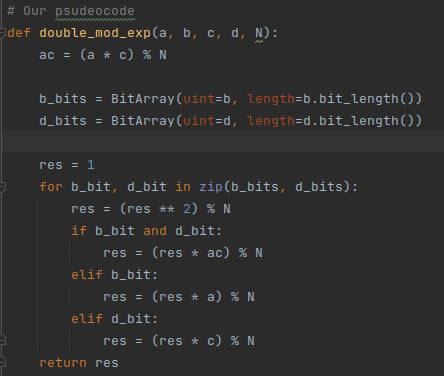
\includegraphics[scale=0.5]{p1_code.png}\\
My algorithm, in the worst case (where $b = c = 2^{n} - 1$), makes $2n + 1$ calls to $MUL$ and $2n + 1$ calls to $MOD$.
\\\\
It is correct because in all cases it multiples $res$ by the correct combination of $a$ and $c$ according to each's respective exponent.
\section{2}
\subsection{a}
The best case runtime occurs when $2^{n - 1} \geq b = 2^{n - 1} < 2^{n}$. In this case, $b_2 = 1 || 0^{n-1}$ and only one bit of $b$ is set to $1$. Therefore $MOD-EXP$ only makes $n + 1$ calls to $MUL$ and $n + 1$ calls to $MOD$.
\subsection{b}
The worst case runtime occurs when $2^{n - 1} \geq b = 2^{n} - 1 < 2^{n}$. In this case, $b_2 = 1^n$ and all the bits of $b$ are set to $1$. Therefore $MOD-EXP$ makes $n + n = 2n$ calls to $MUL$ and $n + n = 2n$ calls to $MOD$.

\section{3}
\subsection{c}
$\mathbb{G}$ is a group
\begin{enumerate}
	\item $\exists e \in \mathbb{G} s.t. \forall g \in \mathbb{G}, e \circ g = g \circ e = g$
		\subitem The identity permutation $e: \Sigma \rightarrow \Sigma s.t. \forall x \in \Sigma, e(x) = x$ is in $\mathbb{G}$, since $e(A) = A$.
		\subitem Moreover $\forall x \in \Sigma, \forall g \in \mathbb{G}, g(e(x)) = g(x) = e(g(x))$
		\subitem Therefore $\forall g \in \mathbb{G}, g \circ e = g = e \circ g$
		\subitem Therefore $e$ is an identity for all $g \in \mathbb{G}$
		\subitem \textbf{QED}
	\item $\forall g \in \mathbb{G}, \exists h \in \mathbb{G} s.t. g \circ h = h \circ g = e$
		\subitem $\forall g \in \mathbb{G}$, with inverse $g^{-1}$, since $g(A) = A$, $g^{-1}(A) = A$. Therefore $\forall g \in \mathbb{G}$, $g^{-1} \in \mathbb{G}$
		\subitem Therefore, $\forall g \in \mathbb{G}, \exists h = g^{-1} \in \mathbb{G} s.t. \forall x \in \Sigma, g(h(x)) = h(g(x)) = e(x)$ (the identity permutation on $\Sigma$)
		\subitem Therefore $\forall g \in \mathbb{G}, \exists h \in \mathbb{G} s.t. g \circ h = h \circ g = e$
		\subitem \textbf{QED}
	\item $\forall g_1, g_2, g_3 \in \mathbb{G}, (g_1 \circ g_2) \circ g_3 = g_1 \circ (g_2 \circ g_3)$. By simplification:
		\subitem $(g_1 \circ g_2) \circ g_3 = g_1 \circ (g_2 \circ g_3)$
		\subitem $\forall x \in \Sigma, g_1(g_2(x)) \circ g_3 = g_1 \circ g_2(g_3(x))$
		\subitem $\forall x \in \Sigma, g_1(g_2(g_3(x))) = g_1(g_2(g_3(x)))$
		\subitem \textbf{QED}
\end{enumerate}

\subsection{d}
$\mathbb{G}$ is \textbf{not} a group
\begin{enumerate}
	\item $\exists e \in \mathbb{G} s.t. \forall g \in \mathbb{G}, e \circ g = g \circ e = g$
		\subitem The identity permutation $e: \Sigma \rightarrow \Sigma s.t. \forall x \in \Sigma, e(x) = x$ is in $\mathbb{G}$. (Given)
		\subitem Moreover $\forall x \in \Sigma, \forall g \in \mathbb{G}, g(e(x)) = g(x) = e(g(x))$
		\subitem Therefore $\forall g \in \mathbb{G}, g \circ e = g = e \circ g$
		\subitem Therefore $e$ is an identity for all $g \in \mathbb{G}$
	\item but, $\not \forall g \in \mathbb{G}, \exists h \in \mathbb{G} s.t. g \circ h = h \circ g = e$
		\subitem Consider two permutations $\sigma, \delta \in \mathbb{G}$ s.t. $\sigma \neq e, \delta \neq e, \sigma \circ \delta = \delta \circ \sigma  = e$ ($\sigma$ and $\delta$ are inverses of one another)
		\subitem This implies that $\forall x \in \Sigma, \sigma(\delta(x)) = \delta(\sigma(x)) = e(x) = x$
		\subitem Therefore, for $x = A$, $\sigma(\delta(A)) = \delta(\sigma(A)) = e$
		\subitem Since for all $g \in \mathbb{G}, g \neq e, g(A) = B$,  $\sigma(B) = \delta(B) = e(A) = A$
		\subitem Observe that for both $\sigma$ and $\delta$, $\sigma(B) = \delta(B) = A$.
		\subitem Therefore, for an member of $g \in \mathbb{G}, g \neq e$ to be invertible, $g(B) = A$
		\subitem Since this is not a quality of all members of $\mathbb{G}$, not all members of $\mathbb{G}$ are invertible
		\subitem \textbf{QED}
\end{enumerate}

\section{5}
Consider any $m_0, m_1, c \in \mathbb{G}$, and some uniform random variable $\textbf{k}$ on $\mathbb{G}$. Since $m_0, m_1, c$ are constants, we can say that:
\begin{enumerate}
	\item $Pr[\textbf{k} = c \circ m_0^{-1}] = Pr[\textbf{k} = c \circ m_1^{-1}] = \frac{1}{|\mathbb{G}|}$
	\item $Pr[\textbf{k} \circ m_0 = c \circ m_0^{-1} \circ m_0] = Pr[\textbf{k} \circ m_1 = c \circ m_1^{-1} \circ m_1] = \frac{1}{|\mathbb{G}|}$ (Groups cancel)
	\item $Pr[\textbf{k} \circ m_0 = c \circ e] = Pr[\textbf{k} \circ m_1 = c \circ e] = \frac{1}{|\mathbb{G}|}$ (def of Inverse)
	\item $Pr[\textbf{k} \circ m_0 = c] = Pr[\textbf{k} \circ m_1 = c] = \frac{1}{|\mathbb{G}|}$ (def of Identity)
	\item $Pr[E(\textbf{k}, m_0) = c] = Pr[E(\textbf{k}, m_1) = c] = \frac{1}{|\mathbb{G}|}$ (def of E)
\end{enumerate}
Therefore $E$ meets our definition of perfect secrecy.

\section{6}
Proof Steps:
\begin{enumerate}
	\item First we combine all the elements in our group, and set it equivalent to itself:
	\subitem $g_1 \circ g_2 \circ ... \circ g_m = g_1 \circ g_2 \circ ... \circ g_m$ (valid)
	\item Because our group is abelian we reorder one side of our equation to put inverses next to each other:
	\subitem $g_1 \circ g_2 \circ ... \circ g_m = g_7 \circ g_m \circ ... \circ g_2$ (NOT valid)
	\subitem Members of our group, besides our identity, can be inverses of themselves, in which case there is no way to place such members adjacent to their inverses. Reordering therefore does not cause the equation to cancel to the identity $e$.
\end{enumerate}
\section{9}
The size of $|\mathbb{Z}^*_N|$, for $N = pq,$ = $pq - p - q + 1$. Therefore the probability of uniformly randomly picking an element $\in \{0, 1, ..., N -1\}$ that is not in $\mathbb{Z}^*_N$ is:
\\\\
$1 - Pr[$picking an element in $\mathbb{Z}^*_N] = 1 - \frac{pq - p - q + 1}{pq} = \frac{pq - (pq - p - q + 1)}{pq} = \frac{p + q - 1}{pq} \approx \frac{p + q}{pq} = \frac{p}{pq} + \frac{q}{pq} = \frac{1}{q} + \frac{1}{p}$
\\\\
Therefore when $p$ and $q$ are large (1024 bits long) the probability of choosing a value not in $\mathbb{Z}^*_N$ is $\approx \frac{1}{2^{1024} - 1} + \frac{1}{2^{1024} - 1} \approx 2 * \frac{1}{2^{1024}} \approx 2^{-1023}$

\end{document}